\section{Theoretical Analysis}
\label{sec:analysis}

In this section, the circuit shown in Figure~\ref{fig:Circuit_Base} is analyzed theoretically with the Mesh Method and with the Nodal Method, in order to complement each other results.

\subsection{Mesh Method}

The Mesh Method consists in introducing currents that circulate in the meshes of the circuit, which are the loops that do not contain other loops, as shown in Figure~\ref{fig:Circuit_Mesh}, and then evaluate the circuit based on the new currents.
\begin{figure}[h] \centering
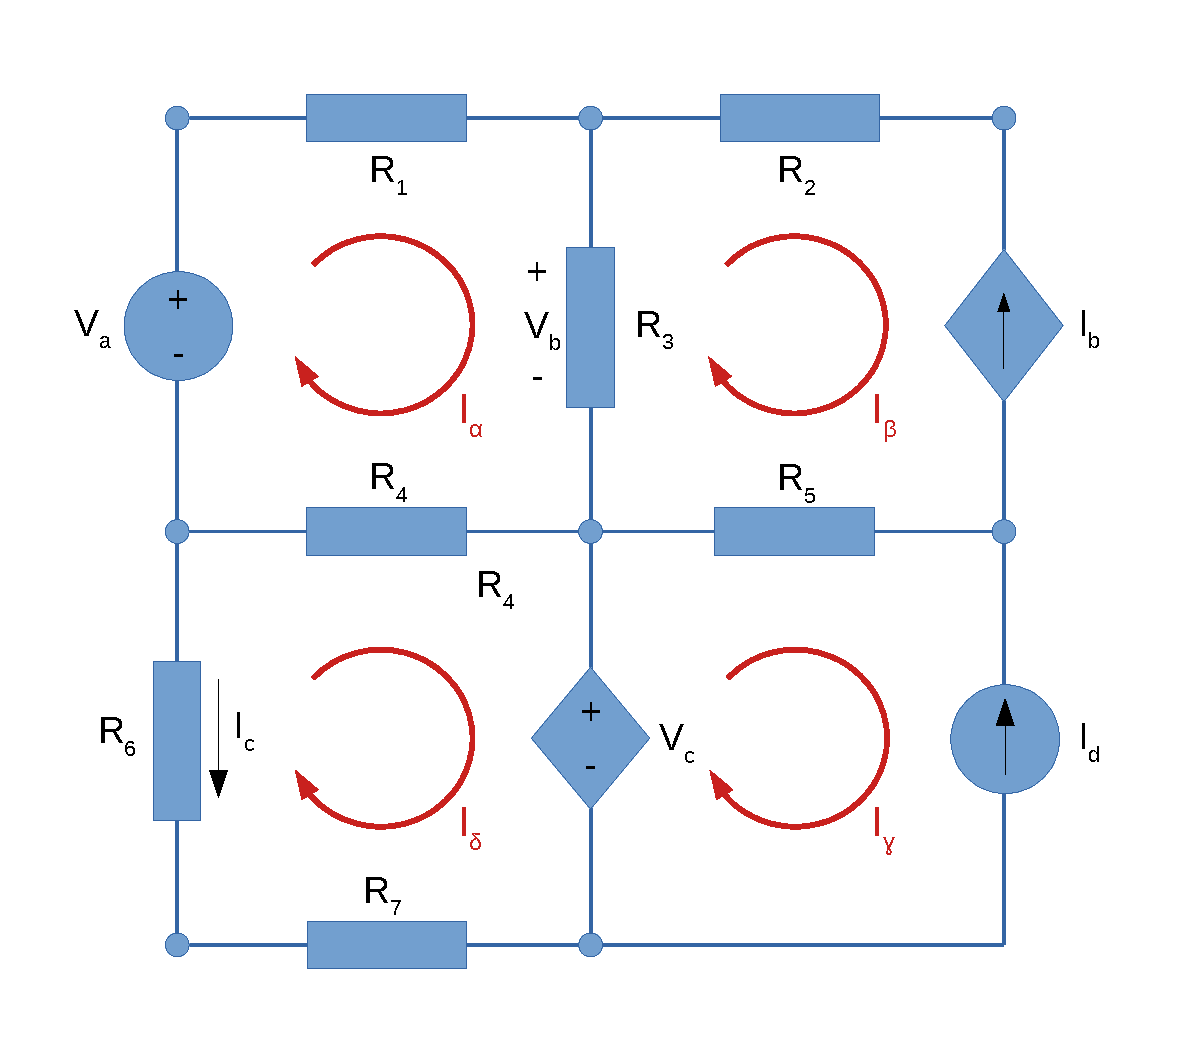
\includegraphics[width=0.45\linewidth]{CircuitMesh.pdf}
\caption{Circuit analysed with mesh currents.}
\label{fig:Circuit_Mesh}
\end{figure}

After identifying the mesh currents, the next step in this method is to use the Kirchhoff Voltage Law~(KVL) in the meshes that do not contain current sources (mesh~$\alpha$~(\ref{eq:MM_Alpha}) and $\delta$~(\ref{eq:MM_Delta})) and to relate the mesh currents to the currents imposed by the sources (mesh~$\beta$~(\ref{eq:MM_Beta}) and $\gamma$~(\ref{eq:MM_Gamma})):
\begin{equation}
  R_1I_{\alpha} + R_3(I_{\alpha}-I_{\beta}) + R_4(I_{\alpha}-I_{\delta}) - V_a = 0;
  \label{eq:MM_Alpha}
\end{equation}
\begin{equation}
  I_{\beta} = - I_b;
  \label{eq:MM_Beta}
\end{equation}
\begin{equation}
  I_{\gamma} = - I_d.
  \label{eq:MM_Gamma}
\end{equation}
\begin{equation}
  R_6I_{\delta} + R_4(I_{\delta}-I_{\alpha}) + V_c + R_7I_{\delta} = 0;
  \label{eq:MM_Delta}
\end{equation}

Since there are 8 variables in the circuit, $I_{\alpha}$, $I_{\beta}$, $I_{\gamma}$, $I_{\delta}$, $V_b$, $V_c$, $I_b$, $I_c$, there must be more four independent equations: two of them are already given,

\begin{equation}
  I_b = K_bV_b;
  \label{eq:Vb_Ib}
\end{equation}
\begin{equation}
  V_c = K_cI_c.
  \label{eq:Vc_Ic}
\end{equation}

The other two are found by examining the circuit and with Ohm's Law:

\begin{equation}
  I_c = - I_{\delta};
  \label{eq:MM_Ic}
\end{equation}
\begin{equation}
  V_b = R_3(I_{\alpha}-I_{\beta})
  \label{eq:MM_Vb}
\end{equation}

In resume, the linear system of equations is:
%	IMPORTANTE VER AS MALHAS
%	AS PRIMEIRAS 4 EQUAÇÕES SÃO DOS NÓS ALFA A DELTA, POR ORDEM ALFABETICA
%	AS EQUAÇÕES 5 E 6 SÃO AS RELAÇÕES NO CIRCUITO COM AS FONTES LINEARES
%	AS EQUAÇÕES 7 E 8 SÃO AS RELAÇÕES QUE EXISTEM NAS FONTES LINEARES 
\begin{equation}
\begin{cases}
	(R_1+R_3+R_4)I_{\alpha} - R_3I_{\beta} - R_4I_{\delta} &= V_a;		\\
  	I_{\beta} + I_b &= 0;												\\
  	I_{\gamma} &= - I_d.												\\
  	(R_6+R_4+R_7)I_{\delta} - R_4I_{\alpha} + V_c &= 0;					\\
  	I_{\delta} + I_c &= 0; 												\\
  	R_3I_{\alpha} - R_3I_{\beta} - V_b &= 0.							\\
  	-K_bV_b + I_b &= 0;													\\
  	V_c - K_cI_c &= 0.
\end{cases}
\end{equation}

The solution to this linear system of equations is determined by Octave:
\begin{table}[h]
  \centering
  \begin{tabular}{|l|r|}
    \hline    
    {\bf Name} & {\bf Value [A or V]} \\ \hline
    \input{../mat/Malhas_tab}
  \end{tabular}
  \caption{Variables in the Mesh Method. A variable preceded by @ is of type {\em current} and expressed in Ampere; other variables are of type {\em voltage} and expressed in Volt.}
  \label{tab:malhas}
\end{table}

\subsection{Nodal Method}

Firstly, computing the values of current and voltage using the nodal method requires finding all the knots in the circuit, as it is presented in Figure \ref{fig:Circuit_Nodal}.
\begin{figure}[h] \centering
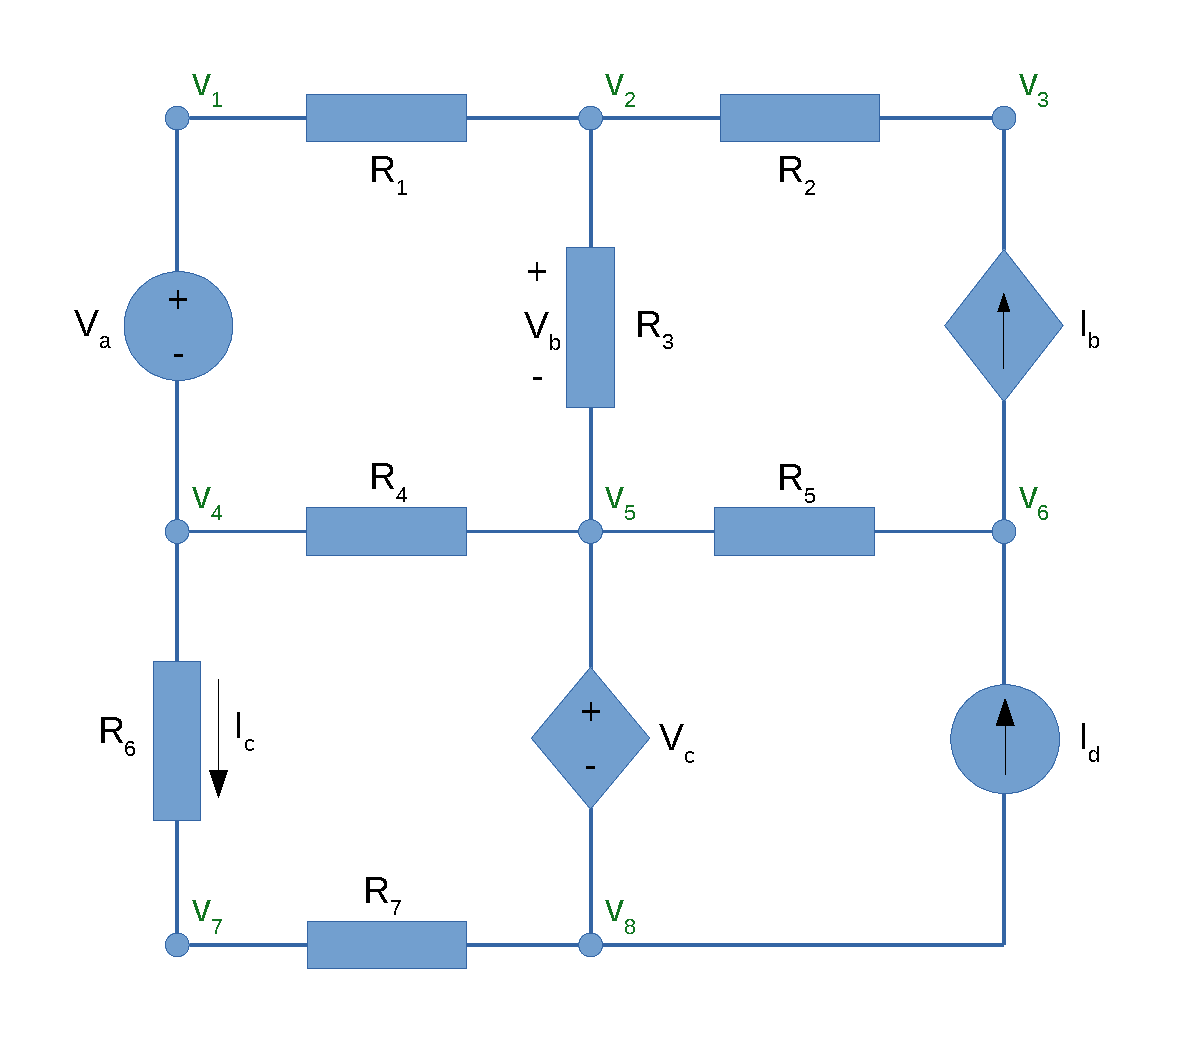
\includegraphics[width=0.5\linewidth]{CircuitNodal.pdf}
\caption{Circuit analysed with nodal voltages.}
\label{fig:Circuit_Nodal}
\end{figure}

Then, the Kirchhoff Current Law~(KCL) is used in the nodes not connected to voltage sources (Equations~\ref{eq:NM_Point2}~to~\ref{eq:NM_Point7}) and two additional equations relating the knots voltages with the voltage sources connected to them are presented (Equations~\ref{eq:NM_Va}~and~\ref{eq:NM_Vc}):

\begin{equation}
  \frac{v_3-v_2}{R_2} + \frac{v_2-v_5}{R_3} + \frac{v_1-v_2}{R_1} = 0;
  \label{eq:NM_Point2}
\end{equation}
\begin{equation}
  I_b + \frac{v_2-v_3}{R_2} = 0;	
  \label{eq:NM_Point3}
\end{equation}
\begin{equation}
  \frac{v_5-v_6}{R_5} - I_b + I_d = 0;
  \label{eq:NM_Point6}
\end{equation}
\begin{equation}
  \frac{v_4-v_7}{R_6} + \frac{v_8-v_7}{R_7} = 0;
  \label{eq:NM_Point7}
\end{equation}

\begin{equation}
  v_1 - v_4 = V_a;
  \label{eq:NM_Va}
\end{equation}
\begin{equation}
  v_5 - v_8 = V_c.
  \label{eq:NM_Vc}
\end{equation}

Since there are 8+4 variables ($v_1$~to~$v_8$, $V_b$, $V_c$, $I_b$, $I_c$), the system is defined by twelve independent equations. Two are provided in the circuit and are the same as in the Mesh Method, (\ref{eq:Vb_Ib})~and~(\ref{eq:Vc_Ic}).
By observing the circuit,
\begin{equation}
  v_2 - v_5 = V_b.
  \label{eq:NM_Vb}
\end{equation}

Using Ohm’s Law, the following relation is found:
\begin{equation}
  \frac{v_4-v_7}{R_6} = I_c.
  \label{eq:NM_OhmIc}
\end{equation}

Because there needs to be a knot with a defined voltage, we chose $v_4$ to be connected to the ground:
\begin{equation}
  v_4 = 0.
  \label{eq:NM_v4=0}
\end{equation}

For the last equation, the continuity of current in the circuit can be used to create a “super-knot”, bypassing the voltage sources $V_a$ and $V_c$, from which the equations are~(\ref{eq:NM_SPVa}) and~(\ref{eq:NM_SPVc}), respectively:

\begin{equation}
  \frac{v_5-v_4}{R_4} + \frac{v_2-v_1}{R_1} - \frac{v_4-v_7}{R_6} = 0;
  \label{eq:NM_SPVa}
\end{equation}
\begin{equation}
  \frac{v_7-v_8}{R_7} - Id + \frac{v_6-v_5}{R_5} + \frac{v_2-v_5}{R_3} + \frac{v_4-v_5}{R_4} = 0.
  \label{eq:NM_SPVc}
\end{equation}

Given that only one more equation is needed, we chose to use the simpler one~(\ref{eq:NM_SPVa}).
%	IMPORTANTE VER OS NÓS
%	AS PRIMEIRAS 7 EQUAÇÕES SÃO DOS NÓS 1 A 7, EM QUE O PRIMEIRO NÓ COM UMA FONTE DE TENSÃO MOSTRA A RELAÇÃO ENTRE OS NÓS EXTREMOS, A SEGUNDA (DO OUTRO NÓ) FAZ A EQUAÇÃO DO SUPERNÓ
%	AS EQUAÇÕES 8 E 9 SÃO AS RELAÇÕES NO CIRCUITO COM AS FONTES LINEARES
%	A EQUAÇÃO 10 É O ZERO DOS NÓS
%	AS EQUAÇÕES 11 E 12 SÃO AS RELAÇÕES QUE EXISTEM NAS FONTES LINEARES 

\begin{equation}
\begin{cases}
	v_1 - v_4 &= V_a;																				  \\
	\frac{1}{R_1}v_1 - (\frac{1}{R_2}+\frac{1}{R_1}+\frac{1}{R_3})v_2 + (\frac{1}{R_2})v_3 + \frac{1}{R_3}v_5 &= 0; \\
  	\frac{1}{R_2}v_2 - \frac{1}{R_2}v_3+ I_b &= 0;													  \\
  	-\frac{1}{R_1}v_1 + \frac{1}{R_1}v_2 - (\frac{1}{R_4}+\frac{1}{R_6})v_4 + \frac{1}{R_4}v_5 + \frac{1}{R_6}v_7 &= 0;			  																	  \\
	v_5 - v_8 - V_c &= 0;																			  \\
  	\frac{1}{R_5}v_5 - \frac{1}{R_5}v_6 - I_b &= -I_d;												  \\
  	-(\frac{1}{R_7}+\frac{1}{R_6})v_7 + \frac{1}{R_7}v_8 + \frac{1}{R_6}v_4 &= 0;					  \\
	v_2 - v_3 - V_b &= 0;																			  \\
  	\frac{1}{R_6}v_4 - \frac{1}{R_6}v_7 - I_c &= 0;													  \\
  	v_4 &= 0;																						  \\
  	-K_bV_b + I_b &= 0;																				  \\
  	V_c - K_cI_c &= 0.
\end{cases}
\end{equation}

The solution to this linear system of equations is determined by Octave:

\begin{table}[h]
  \centering
  \begin{tabular}{|l|r|}
  \hline  
    {\bf Name} & {\bf Value [A or V]} \\ \hline
    \input{../mat/Nos_tab}
  \end{tabular}
  \caption{Variables in the Nodal Method. A variable preceded by @ is of type {\em current} and expressed in Ampere; other variables are of type {\em voltage} and expressed in Volt.}
  \label{tab:nos}
\end{table}

